\documentclass[]{article}
\usepackage{lmodern}
\usepackage{amssymb,amsmath}
\usepackage{ifxetex,ifluatex}
\usepackage{fixltx2e} % provides \textsubscript
\ifnum 0\ifxetex 1\fi\ifluatex 1\fi=0 % if pdftex
  \usepackage[T1]{fontenc}
  \usepackage[utf8]{inputenc}
\else % if luatex or xelatex
  \ifxetex
    \usepackage{mathspec}
  \else
    \usepackage{fontspec}
  \fi
  \defaultfontfeatures{Ligatures=TeX,Scale=MatchLowercase}
\fi
% use upquote if available, for straight quotes in verbatim environments
\IfFileExists{upquote.sty}{\usepackage{upquote}}{}
% use microtype if available
\IfFileExists{microtype.sty}{%
\usepackage{microtype}
\UseMicrotypeSet[protrusion]{basicmath} % disable protrusion for tt fonts
}{}
\usepackage[margin=1in]{geometry}
\usepackage{hyperref}
\hypersetup{unicode=true,
            pdftitle={Final Project - Analyzing Use of Verbs in Tweets},
            pdfauthor={Deanna Schneider},
            pdfborder={0 0 0},
            breaklinks=true}
\urlstyle{same}  % don't use monospace font for urls
\usepackage{color}
\usepackage{fancyvrb}
\newcommand{\VerbBar}{|}
\newcommand{\VERB}{\Verb[commandchars=\\\{\}]}
\DefineVerbatimEnvironment{Highlighting}{Verbatim}{commandchars=\\\{\}}
% Add ',fontsize=\small' for more characters per line
\usepackage{framed}
\definecolor{shadecolor}{RGB}{248,248,248}
\newenvironment{Shaded}{\begin{snugshade}}{\end{snugshade}}
\newcommand{\KeywordTok}[1]{\textcolor[rgb]{0.13,0.29,0.53}{\textbf{#1}}}
\newcommand{\DataTypeTok}[1]{\textcolor[rgb]{0.13,0.29,0.53}{#1}}
\newcommand{\DecValTok}[1]{\textcolor[rgb]{0.00,0.00,0.81}{#1}}
\newcommand{\BaseNTok}[1]{\textcolor[rgb]{0.00,0.00,0.81}{#1}}
\newcommand{\FloatTok}[1]{\textcolor[rgb]{0.00,0.00,0.81}{#1}}
\newcommand{\ConstantTok}[1]{\textcolor[rgb]{0.00,0.00,0.00}{#1}}
\newcommand{\CharTok}[1]{\textcolor[rgb]{0.31,0.60,0.02}{#1}}
\newcommand{\SpecialCharTok}[1]{\textcolor[rgb]{0.00,0.00,0.00}{#1}}
\newcommand{\StringTok}[1]{\textcolor[rgb]{0.31,0.60,0.02}{#1}}
\newcommand{\VerbatimStringTok}[1]{\textcolor[rgb]{0.31,0.60,0.02}{#1}}
\newcommand{\SpecialStringTok}[1]{\textcolor[rgb]{0.31,0.60,0.02}{#1}}
\newcommand{\ImportTok}[1]{#1}
\newcommand{\CommentTok}[1]{\textcolor[rgb]{0.56,0.35,0.01}{\textit{#1}}}
\newcommand{\DocumentationTok}[1]{\textcolor[rgb]{0.56,0.35,0.01}{\textbf{\textit{#1}}}}
\newcommand{\AnnotationTok}[1]{\textcolor[rgb]{0.56,0.35,0.01}{\textbf{\textit{#1}}}}
\newcommand{\CommentVarTok}[1]{\textcolor[rgb]{0.56,0.35,0.01}{\textbf{\textit{#1}}}}
\newcommand{\OtherTok}[1]{\textcolor[rgb]{0.56,0.35,0.01}{#1}}
\newcommand{\FunctionTok}[1]{\textcolor[rgb]{0.00,0.00,0.00}{#1}}
\newcommand{\VariableTok}[1]{\textcolor[rgb]{0.00,0.00,0.00}{#1}}
\newcommand{\ControlFlowTok}[1]{\textcolor[rgb]{0.13,0.29,0.53}{\textbf{#1}}}
\newcommand{\OperatorTok}[1]{\textcolor[rgb]{0.81,0.36,0.00}{\textbf{#1}}}
\newcommand{\BuiltInTok}[1]{#1}
\newcommand{\ExtensionTok}[1]{#1}
\newcommand{\PreprocessorTok}[1]{\textcolor[rgb]{0.56,0.35,0.01}{\textit{#1}}}
\newcommand{\AttributeTok}[1]{\textcolor[rgb]{0.77,0.63,0.00}{#1}}
\newcommand{\RegionMarkerTok}[1]{#1}
\newcommand{\InformationTok}[1]{\textcolor[rgb]{0.56,0.35,0.01}{\textbf{\textit{#1}}}}
\newcommand{\WarningTok}[1]{\textcolor[rgb]{0.56,0.35,0.01}{\textbf{\textit{#1}}}}
\newcommand{\AlertTok}[1]{\textcolor[rgb]{0.94,0.16,0.16}{#1}}
\newcommand{\ErrorTok}[1]{\textcolor[rgb]{0.64,0.00,0.00}{\textbf{#1}}}
\newcommand{\NormalTok}[1]{#1}
\usepackage{graphicx,grffile}
\makeatletter
\def\maxwidth{\ifdim\Gin@nat@width>\linewidth\linewidth\else\Gin@nat@width\fi}
\def\maxheight{\ifdim\Gin@nat@height>\textheight\textheight\else\Gin@nat@height\fi}
\makeatother
% Scale images if necessary, so that they will not overflow the page
% margins by default, and it is still possible to overwrite the defaults
% using explicit options in \includegraphics[width, height, ...]{}
\setkeys{Gin}{width=\maxwidth,height=\maxheight,keepaspectratio}
\IfFileExists{parskip.sty}{%
\usepackage{parskip}
}{% else
\setlength{\parindent}{0pt}
\setlength{\parskip}{6pt plus 2pt minus 1pt}
}
\setlength{\emergencystretch}{3em}  % prevent overfull lines
\providecommand{\tightlist}{%
  \setlength{\itemsep}{0pt}\setlength{\parskip}{0pt}}
\setcounter{secnumdepth}{0}
% Redefines (sub)paragraphs to behave more like sections
\ifx\paragraph\undefined\else
\let\oldparagraph\paragraph
\renewcommand{\paragraph}[1]{\oldparagraph{#1}\mbox{}}
\fi
\ifx\subparagraph\undefined\else
\let\oldsubparagraph\subparagraph
\renewcommand{\subparagraph}[1]{\oldsubparagraph{#1}\mbox{}}
\fi

%%% Use protect on footnotes to avoid problems with footnotes in titles
\let\rmarkdownfootnote\footnote%
\def\footnote{\protect\rmarkdownfootnote}

%%% Change title format to be more compact
\usepackage{titling}

% Create subtitle command for use in maketitle
\providecommand{\subtitle}[1]{
  \posttitle{
    \begin{center}\large#1\end{center}
    }
}

\setlength{\droptitle}{-2em}

  \title{Final Project - Analyzing Use of Verbs in Tweets}
    \pretitle{\vspace{\droptitle}\centering\huge}
  \posttitle{\par}
    \author{Deanna Schneider}
    \preauthor{\centering\large\emph}
  \postauthor{\par}
      \predate{\centering\large\emph}
  \postdate{\par}
    \date{October 20, 2017}


\begin{document}
\maketitle

\subsection{Step One - Read in the data that was output from Sentiment
Analysis.ipynb, clean it, and sample
it}\label{step-one---read-in-the-data-that-was-output-from-sentiment-analysis.ipynb-clean-it-and-sample-it}

Two files were generated: metoo\_cleaned.csv and takeaknee\_cleaned.csv
- each of which contained between 7000 and 1800 tweets, collected on
10/26/17 and 12/04/17. Collected data was analyzed in Python and
exported with the addition of sentiment and verb counts.

Each data set has more than the number of tweets I ultimately want
(5000). In the following steps, I will make sure that we have only
full-text tweets, only 1 tweet per author, all unique tweets, remove
non-native English speakers, and verify that there is some content left
in the tweet after it had been cleaned with the regular expression in
Python. After cleaning the tweets, I will get a random set of 5000
tweets from each hashtag.

\begin{Shaded}
\begin{Highlighting}[]
\NormalTok{pacman}\OperatorTok{::}\KeywordTok{p_load}\NormalTok{(}\StringTok{'tidyverse'}\NormalTok{)}

\CommentTok{#define a function that does all the cleaning in R - Note, code to do this all seperately is FinalProject-babysteps.RMD}
\NormalTok{clean_data <-}\StringTok{ }\ControlFlowTok{function}\NormalTok{(filename, }\DataTypeTok{seed =} \DecValTok{71}\NormalTok{, }\DataTypeTok{samplesize =} \DecValTok{5000}\NormalTok{)\{}
  \CommentTok{#The file Utilities.R includes timings for read.csv, scan, and tidyverse's read_csv. Read_csv is the winner.}
  \KeywordTok{library}\NormalTok{(tidyverse)}
  \CommentTok{#read in the file}
\NormalTok{  out_data =}\StringTok{ }\KeywordTok{read_csv}\NormalTok{(filename)}
  \CommentTok{#remove truncated tweets}
\NormalTok{  out_data <-}\StringTok{ }\NormalTok{out_data[}\KeywordTok{which}\NormalTok{(out_data[}\StringTok{"truncated"}\NormalTok{]}\OperatorTok{==}\StringTok{'FALSE'}\NormalTok{), ]}

  \CommentTok{#get unique authors}
\NormalTok{  out_data <-}\StringTok{ }\NormalTok{out_data[}\OperatorTok{!}\KeywordTok{duplicated}\NormalTok{(out_data}\OperatorTok{$}\NormalTok{AuthorID),]}
  \CommentTok{#get unique tweets}
\NormalTok{  out_data <-}\StringTok{ }\NormalTok{out_data[}\OperatorTok{!}\KeywordTok{duplicated}\NormalTok{(out_data}\OperatorTok{$}\NormalTok{Text),]}
  \CommentTok{#get only native English Speakers}
\NormalTok{  out_data <-}\StringTok{ }\NormalTok{out_data[out_data}\OperatorTok{$}\NormalTok{Language }\OperatorTok{==}\StringTok{ 'en'}\NormalTok{,]}
  \CommentTok{#make sure there's something in the clean tweet}
\NormalTok{  out_data <-}\StringTok{ }\NormalTok{out_data[}\KeywordTok{length}\NormalTok{(out_data}\OperatorTok{$}\NormalTok{cleanTweet) }\OperatorTok{>}\StringTok{ }\DecValTok{0}\NormalTok{,]}
  \CommentTok{#set a seed}
  \KeywordTok{set.seed}\NormalTok{(seed)}
  \CommentTok{#return a random sample of 5000 tweets}
  
\NormalTok{  out_data <-}\StringTok{ }\NormalTok{out_data[}\KeywordTok{sample}\NormalTok{(}\KeywordTok{nrow}\NormalTok{(out_data), samplesize), ]}
  
  \KeywordTok{return}\NormalTok{(out_data)}
\NormalTok{\}}
\end{Highlighting}
\end{Shaded}

\begin{Shaded}
\begin{Highlighting}[]
\NormalTok{metoo <-}\StringTok{ }\KeywordTok{clean_data}\NormalTok{(}\StringTok{'metoo_cleaned.csv'}\NormalTok{, }\DataTypeTok{samplesize=}\DecValTok{2000}\NormalTok{)}
\NormalTok{metoo_split <-}\StringTok{ }\KeywordTok{clean_data}\NormalTok{(}\StringTok{'metoo_cleaned_split.csv'}\NormalTok{)}
\NormalTok{knee <-}\StringTok{ }\KeywordTok{clean_data}\NormalTok{(}\StringTok{'takeaknee_cleaned.csv'}\NormalTok{)}
\NormalTok{knee_split <-}\StringTok{ }\KeywordTok{clean_data}\NormalTok{(}\StringTok{'takeaknee_cleaned_split.csv'}\NormalTok{)}
\KeywordTok{dim}\NormalTok{(metoo)}
\KeywordTok{dim}\NormalTok{(metoo_split)}
\KeywordTok{dim}\NormalTok{(knee)}
\KeywordTok{dim}\NormalTok{(knee_split)}
\end{Highlighting}
\end{Shaded}

\begin{Shaded}
\begin{Highlighting}[]
\CommentTok{#fetch a random sample from each dataset, for Table 1}
\CommentTok{#set the seed (so this can be reproduced)}
\KeywordTok{set.seed}\NormalTok{(}\DecValTok{71}\NormalTok{)}

\NormalTok{metoo_tweet <-}\StringTok{ }\NormalTok{metoo[}\KeywordTok{sample}\NormalTok{(}\KeywordTok{nrow}\NormalTok{(metoo), }\DecValTok{1}\NormalTok{), ]}
\NormalTok{knee_tweet <-}\StringTok{ }\NormalTok{knee[}\KeywordTok{sample}\NormalTok{(}\KeywordTok{nrow}\NormalTok{(knee), }\DecValTok{1}\NormalTok{), ]}

\KeywordTok{print}\NormalTok{(}\KeywordTok{paste}\NormalTok{(metoo_tweet}\OperatorTok{$}\NormalTok{AuthorID, }\StringTok{' - '}\NormalTok{, metoo_tweet}\OperatorTok{$}\NormalTok{cleanTweet))}
\end{Highlighting}
\end{Shaded}

\begin{verbatim}
## [1] "221031253  -  two colleges bound by history are roiled by the metoo moment"
\end{verbatim}

\begin{Shaded}
\begin{Highlighting}[]
\KeywordTok{print}\NormalTok{(}\KeywordTok{paste}\NormalTok{(knee_tweet}\OperatorTok{$}\NormalTok{AuthorID, }\StringTok{' - '}\NormalTok{, knee_tweet}\OperatorTok{$}\NormalTok{cleanTweet))}
\end{Highlighting}
\end{Shaded}

\begin{verbatim}
## [1] "899809169221365760  -  takeaknee just stand up"
\end{verbatim}

\subsection{Step Three - Review Verb
Distribution}\label{step-three---review-verb-distribution}

In order to use a t.test, we need to have a sizable sample (requirement
met), and ideally have a normal distribution. In the following code
cells, I produce histograms of the data to review the distributions. I
also review the distribution of the logged data.

\begin{Shaded}
\begin{Highlighting}[]
\CommentTok{#look at the distribution of verbs in each dataset}
\KeywordTok{hist}\NormalTok{(metoo}\OperatorTok{$}\NormalTok{total_verbs, }\DataTypeTok{main=}\StringTok{"Hashtagged Verb Distributions (Overlaid)"}\NormalTok{, }\DataTypeTok{xlab=}\StringTok{"Total Verbs"}\NormalTok{, }\DataTypeTok{col=}\StringTok{'skyblue4'}\NormalTok{, }\DataTypeTok{ylim=}\KeywordTok{c}\NormalTok{(}\DecValTok{0}\NormalTok{, }\DecValTok{2100}\NormalTok{))}
\KeywordTok{hist}\NormalTok{(knee}\OperatorTok{$}\NormalTok{total_verbs, }\DataTypeTok{col=}\StringTok{'#8B7B8B7F'}\NormalTok{, }\DataTypeTok{ylim=}\KeywordTok{c}\NormalTok{(}\DecValTok{0}\NormalTok{,}\DecValTok{2100}\NormalTok{), }\DataTypeTok{add=}\NormalTok{T)}
\KeywordTok{legend}\NormalTok{(}\StringTok{"topright"}\NormalTok{, }\KeywordTok{c}\NormalTok{(}\StringTok{'#takeaknee'}\NormalTok{, }\StringTok{'#metoo'}\NormalTok{), }\DataTypeTok{fill=}\KeywordTok{c}\NormalTok{(}\StringTok{'#8B7B8B7F'}\NormalTok{, }\StringTok{'skyblue4'}\NormalTok{))}
\end{Highlighting}
\end{Shaded}

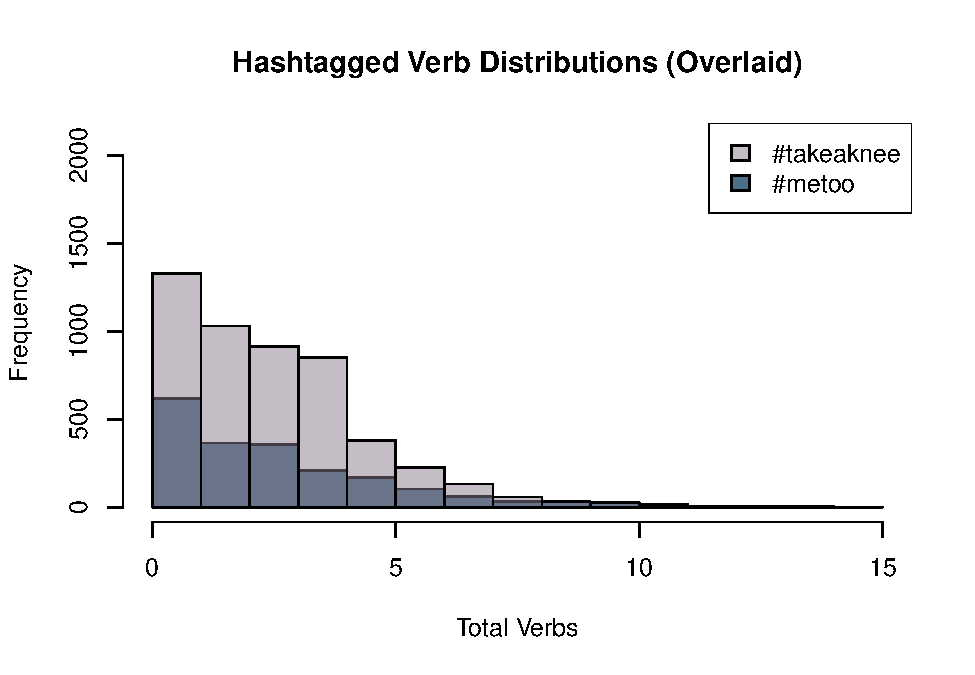
\includegraphics{figure/hist_total_verbs_overlaid-1.pdf}

\begin{Shaded}
\begin{Highlighting}[]
\CommentTok{#look at the distribution of verbs in each dataset}
\KeywordTok{hist}\NormalTok{(metoo_split}\OperatorTok{$}\NormalTok{total_verbs, }\DataTypeTok{main=}\StringTok{"Individual Word Verb Distributions (Overlaid)"}\NormalTok{, }\DataTypeTok{xlab=}\StringTok{"Total Verbs"}\NormalTok{, }\DataTypeTok{col=}\StringTok{'skyblue4'}\NormalTok{, }\DataTypeTok{ylim=}\KeywordTok{c}\NormalTok{(}\DecValTok{0}\NormalTok{, }\DecValTok{2100}\NormalTok{))}
\KeywordTok{hist}\NormalTok{(knee_split}\OperatorTok{$}\NormalTok{total_verbs, }\DataTypeTok{col=}\StringTok{'#8B7B8B7F'}\NormalTok{, }\DataTypeTok{ylim=}\KeywordTok{c}\NormalTok{(}\DecValTok{0}\NormalTok{,}\DecValTok{2100}\NormalTok{), }\DataTypeTok{add=}\NormalTok{T)}
\KeywordTok{legend}\NormalTok{(}\StringTok{"topright"}\NormalTok{, }\KeywordTok{c}\NormalTok{(}\StringTok{'take a knee'}\NormalTok{, }\StringTok{'me too'}\NormalTok{), }\DataTypeTok{fill=}\KeywordTok{c}\NormalTok{(}\StringTok{'#8B7B8B7F'}\NormalTok{, }\StringTok{'skyblue4'}\NormalTok{))}
\end{Highlighting}
\end{Shaded}

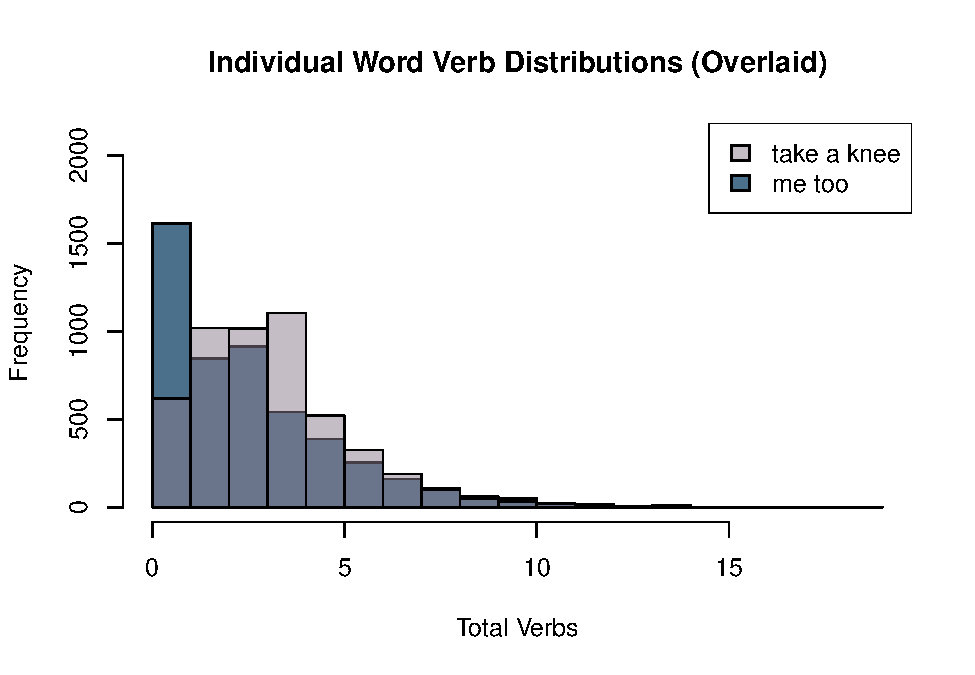
\includegraphics{figure/hist_total_verbs_split_overlaid-1.pdf}

\begin{Shaded}
\begin{Highlighting}[]
\CommentTok{#Anything over 10 verbs seems like a lot for 140 characters. Let's do a sanity check on those. }

\NormalTok{metoo[}\KeywordTok{which}\NormalTok{(metoo}\OperatorTok{$}\NormalTok{total_verbs }\OperatorTok{>}\StringTok{ }\DecValTok{10}\NormalTok{), ]}
\NormalTok{knee[}\KeywordTok{which}\NormalTok{(knee}\OperatorTok{$}\NormalTok{total_verbs }\OperatorTok{>}\StringTok{ }\DecValTok{10}\NormalTok{), ]}
\end{Highlighting}
\end{Shaded}

\subsubsection{Step Three-A}\label{step-three-a}

The sanity check indicates that there really are legitimate tweets with
a large number of verbs. I also visually inspected the zero verb tweets
in Excel. I considered removing the zero verb tweets, but they are also
a legitimate part of the dataset. So, I chose to leave both ends of the
spectrum in the data.

\begin{Shaded}
\begin{Highlighting}[]
\CommentTok{#look at the distribution of logged verbs in each dataset. This is going to be remarkably simiar between the split and not split, so just do it for the not split datasets.}
\KeywordTok{par}\NormalTok{(}\DataTypeTok{mfrow=}\KeywordTok{c}\NormalTok{(}\DecValTok{1}\NormalTok{,}\DecValTok{2}\NormalTok{))}

\KeywordTok{hist}\NormalTok{(}\KeywordTok{log}\NormalTok{(knee}\OperatorTok{$}\NormalTok{total_verbs), }\DataTypeTok{main=}\StringTok{"#takeaknee Logged Verb Distribution"}\NormalTok{, }\DataTypeTok{xlab=}\StringTok{"Total Logged Verbs"}\NormalTok{, }\DataTypeTok{col=}\StringTok{'thistle4'}\NormalTok{)}
\KeywordTok{hist}\NormalTok{(}\KeywordTok{log}\NormalTok{(metoo}\OperatorTok{$}\NormalTok{total_verbs), }\DataTypeTok{main=}\StringTok{"#metoo Logged Verb Distribution"}\NormalTok{, }\DataTypeTok{xlab=}\StringTok{"Total Logged Verbs"}\NormalTok{,}\DataTypeTok{col=}\StringTok{'skyblue4'}\NormalTok{)}
\end{Highlighting}
\end{Shaded}

\includegraphics{FinalProject-R_files/figure-latex/hist_log_total_verbs-1.pdf}

\subsection{Step Four - Decision on Distribution
Appropriateness}\label{step-four---decision-on-distribution-appropriateness}

The data for verb count is clearly heavily skewed. While the sample size
is large enough to use a t-test, the distribution would suggest using a
Wilcox text instead. Proceed with a both a t-test and a Wilcoxon test.
Hopefully, the results will match.

\subsection{Step Five - Prepare for and Complete a
T-Test}\label{step-five---prepare-for-and-complete-a-t-test}

\begin{Shaded}
\begin{Highlighting}[]
\CommentTok{#These summaries are just helpful for my own understanding of the data.}
\KeywordTok{print}\NormalTok{(}\StringTok{"Knee - not split"}\NormalTok{)}
\end{Highlighting}
\end{Shaded}

\begin{verbatim}
## [1] "Knee - not split"
\end{verbatim}

\begin{Shaded}
\begin{Highlighting}[]
\KeywordTok{summary}\NormalTok{(knee}\OperatorTok{$}\NormalTok{total_verbs)}
\end{Highlighting}
\end{Shaded}

\begin{verbatim}
##    Min. 1st Qu.  Median    Mean 3rd Qu.    Max. 
##   0.000   1.000   3.000   2.917   4.000  14.000
\end{verbatim}

\begin{Shaded}
\begin{Highlighting}[]
\KeywordTok{print}\NormalTok{(}\StringTok{"Knee - split"}\NormalTok{)}
\end{Highlighting}
\end{Shaded}

\begin{verbatim}
## [1] "Knee - split"
\end{verbatim}

\begin{Shaded}
\begin{Highlighting}[]
\KeywordTok{summary}\NormalTok{(knee_split}\OperatorTok{$}\NormalTok{total_verbs)}
\end{Highlighting}
\end{Shaded}

\begin{verbatim}
##    Min. 1st Qu.  Median    Mean 3rd Qu.    Max. 
##   0.000   2.000   3.000   3.581   4.000  14.000
\end{verbatim}

\begin{Shaded}
\begin{Highlighting}[]
\KeywordTok{print}\NormalTok{(}\StringTok{"Metoo - not split"}\NormalTok{)}
\end{Highlighting}
\end{Shaded}

\begin{verbatim}
## [1] "Metoo - not split"
\end{verbatim}

\begin{Shaded}
\begin{Highlighting}[]
\KeywordTok{summary}\NormalTok{(metoo}\OperatorTok{$}\NormalTok{total_verbs)}
\end{Highlighting}
\end{Shaded}

\begin{verbatim}
##    Min. 1st Qu.  Median    Mean 3rd Qu.    Max. 
##   0.000   1.000   3.000   3.039   4.000  15.000
\end{verbatim}

\begin{Shaded}
\begin{Highlighting}[]
\KeywordTok{print}\NormalTok{(}\StringTok{"Metoo - split"}\NormalTok{)}
\end{Highlighting}
\end{Shaded}

\begin{verbatim}
## [1] "Metoo - split"
\end{verbatim}

\begin{Shaded}
\begin{Highlighting}[]
\KeywordTok{summary}\NormalTok{(metoo_split}\OperatorTok{$}\NormalTok{total_verbs)}
\end{Highlighting}
\end{Shaded}

\begin{verbatim}
##    Min. 1st Qu.  Median    Mean 3rd Qu.    Max. 
##   0.000   1.000   3.000   2.978   4.000  19.000
\end{verbatim}

\begin{Shaded}
\begin{Highlighting}[]
\CommentTok{#do a t test}
\KeywordTok{t.test}\NormalTok{(knee}\OperatorTok{$}\NormalTok{total_verbs, metoo}\OperatorTok{$}\NormalTok{total_verbs, }\DataTypeTok{alternative=}\StringTok{"two.sided"}\NormalTok{)}
\end{Highlighting}
\end{Shaded}

\begin{verbatim}
## 
##  Welch Two Sample t-test
## 
## data:  knee$total_verbs and metoo$total_verbs
## t = -1.9476, df = 3091.2, p-value = 0.05156
## alternative hypothesis: true difference in means is not equal to 0
## 95 percent confidence interval:
##  -0.2454274892  0.0008274892
## sample estimates:
## mean of x mean of y 
##    2.9172    3.0395
\end{verbatim}

\begin{Shaded}
\begin{Highlighting}[]
\CommentTok{#do a t test}
\KeywordTok{t.test}\NormalTok{(knee_split}\OperatorTok{$}\NormalTok{total_verbs, metoo_split}\OperatorTok{$}\NormalTok{total_verbs, }\DataTypeTok{alternative=}\StringTok{"two.sided"}\NormalTok{)}
\end{Highlighting}
\end{Shaded}

\begin{verbatim}
## 
##  Welch Two Sample t-test
## 
## data:  knee_split$total_verbs and metoo_split$total_verbs
## t = 13.571, df = 9543.2, p-value < 2.2e-16
## alternative hypothesis: true difference in means is not equal to 0
## 95 percent confidence interval:
##  0.5159015 0.6900985
## sample estimates:
## mean of x mean of y 
##    3.5808    2.9778
\end{verbatim}

\subsubsection{Step Five Results: T-Test
Results}\label{step-five-results-t-test-results}

The null hypothesis is that the mean use of verbs in the metoo tweets
equals the mean use of verbs in the takeaknee tweets. We have
contradictory results between the two tests. At a significance level of
.01, we do not have evidence of varying significantly when the hashtags
are treated as hashtags, but we do have significant evidence of varying
when the hashtags are treated as individual words.

\subsection{Step Six: Complete a Wilcoxon
Test}\label{step-six-complete-a-wilcoxon-test}

\begin{Shaded}
\begin{Highlighting}[]
\CommentTok{#do a wilcox test}
\CommentTok{#https://www.stat.auckland.ac.nz/~wild/ChanceEnc/Ch10.wilcoxon.pdf}
\KeywordTok{wilcox.test}\NormalTok{(knee}\OperatorTok{$}\NormalTok{total_verbs, metoo}\OperatorTok{$}\NormalTok{total_verbs, }\DataTypeTok{alternative=}\StringTok{"two.sided"}\NormalTok{)}
\end{Highlighting}
\end{Shaded}

\begin{verbatim}
## 
##  Wilcoxon rank sum test with continuity correction
## 
## data:  knee$total_verbs and metoo$total_verbs
## W = 5079600, p-value = 0.2913
## alternative hypothesis: true location shift is not equal to 0
\end{verbatim}

\begin{Shaded}
\begin{Highlighting}[]
\CommentTok{#do a wilcox test}
\CommentTok{#https://www.stat.auckland.ac.nz/~wild/ChanceEnc/Ch10.wilcoxon.pdf}
\KeywordTok{wilcox.test}\NormalTok{(knee_split}\OperatorTok{$}\NormalTok{total_verbs, metoo_split}\OperatorTok{$}\NormalTok{total_verbs, }\DataTypeTok{alternative=}\StringTok{"two.sided"}\NormalTok{)}
\end{Highlighting}
\end{Shaded}

\begin{verbatim}
## 
##  Wilcoxon rank sum test with continuity correction
## 
## data:  knee_split$total_verbs and metoo_split$total_verbs
## W = 15206000, p-value < 2.2e-16
## alternative hypothesis: true location shift is not equal to 0
\end{verbatim}

\begin{Shaded}
\begin{Highlighting}[]
\CommentTok{#if the slopes of notched boxplots overlap, there is not a significant difference in the median. Let's view that.}

\CommentTok{#set up a color palette}
\NormalTok{myColors =}\StringTok{ }\KeywordTok{c}\NormalTok{(}\StringTok{'skyblue4'}\NormalTok{,}\StringTok{'thistle4'}\NormalTok{)}


\KeywordTok{boxplot}\NormalTok{(metoo}\OperatorTok{$}\NormalTok{total_verbs, knee}\OperatorTok{$}\NormalTok{total_verbs,  }\DataTypeTok{notch=}\OtherTok{TRUE}\NormalTok{, }
  \DataTypeTok{names=}\KeywordTok{c}\NormalTok{(}\StringTok{"#metoo"}\NormalTok{,}\StringTok{"#takeaknee"}\NormalTok{),}
  \DataTypeTok{col=}\NormalTok{myColors,}
  \DataTypeTok{main=}\StringTok{"Distribution of Total Verbs (not split)"}\NormalTok{,}
  \DataTypeTok{horizontal =} \OtherTok{TRUE}\NormalTok{)}
\end{Highlighting}
\end{Shaded}

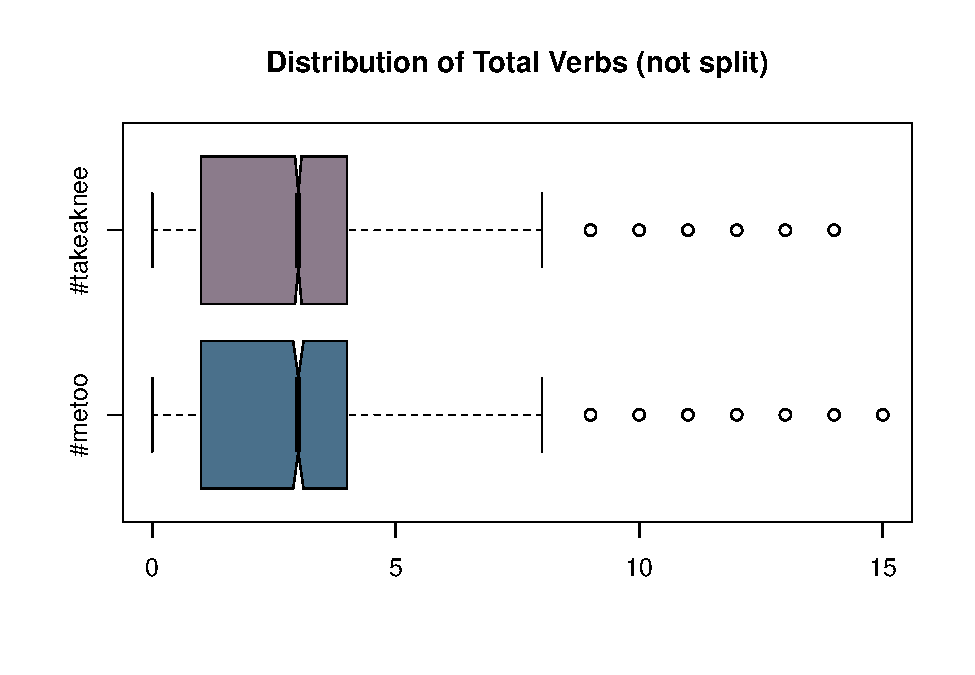
\includegraphics{figure/total_verbs_notched_blox_plot-1.pdf}

\begin{Shaded}
\begin{Highlighting}[]
\KeywordTok{boxplot}\NormalTok{(metoo_split}\OperatorTok{$}\NormalTok{total_verbs, knee_split}\OperatorTok{$}\NormalTok{total_verbs,  }\DataTypeTok{notch=}\OtherTok{TRUE}\NormalTok{, }
  \DataTypeTok{names=}\KeywordTok{c}\NormalTok{(}\StringTok{"me too"}\NormalTok{,}\StringTok{"take a knee"}\NormalTok{),}
  \DataTypeTok{col=}\NormalTok{myColors,}
  \DataTypeTok{main=}\StringTok{"Distribution of Total Verbs (split)"}\NormalTok{,}
  \DataTypeTok{horizontal =} \OtherTok{TRUE}\NormalTok{)}
\end{Highlighting}
\end{Shaded}

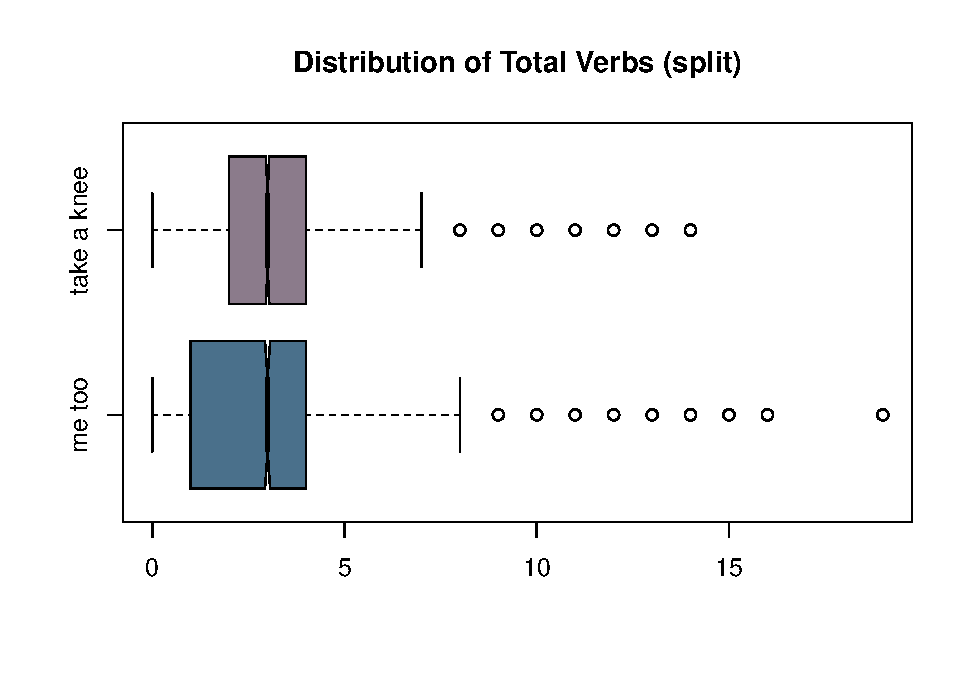
\includegraphics{figure/total_verbs_notched_blox_plot-2.pdf}

\subsubsection{Step Six Results - Results of Wilcoxon
Test}\label{step-six-results---results-of-wilcoxon-test}

The null hypothesis is that the location shift of verbs in each hashtag
is equal to zero. The alternative hypothesis is that the location shift
of verbs is not equal to zero. At the significance level of .01, we see
similar results as the t-test. When the hashtags are treated as
hashtags, there is not enough evidence to assert that the distribution
varies significantly. When the hashtags are treated as individual words,
there is enough evidence to assert that the distributions are of
different shapes. In both instances, the median is the same (3),
indicating that the difference lies truly in the shape of the
distribution, and not in the measure of central tendency.

\subsection{Step Seven - Review Verb
Tense}\label{step-seven---review-verb-tense}

This section could be interesting as a mechanism for further analysis.

\begin{Shaded}
\begin{Highlighting}[]
\NormalTok{verb_cols =}\StringTok{ }\KeywordTok{c}\NormalTok{(}\StringTok{"total_verbs"}\NormalTok{, }\StringTok{"base_verb"}\NormalTok{, }\StringTok{"past_tense"}\NormalTok{,  }\StringTok{"past_participle"}\NormalTok{, }\StringTok{"present_participle"}\NormalTok{, }\StringTok{"present_not_third"}\NormalTok{, }\StringTok{"present_third"}\NormalTok{)}

\NormalTok{metoo_sums =}\StringTok{ }\KeywordTok{apply}\NormalTok{(metoo[verb_cols],}\DecValTok{2}\NormalTok{, sum) }
\NormalTok{knee_sums =}\StringTok{ }\KeywordTok{apply}\NormalTok{(knee[verb_cols],}\DecValTok{2}\NormalTok{, sum)}
\NormalTok{metoo_split_sums =}\StringTok{ }\KeywordTok{apply}\NormalTok{(metoo_split[verb_cols],}\DecValTok{2}\NormalTok{, sum) }
\NormalTok{knee_split_sums =}\StringTok{ }\KeywordTok{apply}\NormalTok{(knee_split[verb_cols],}\DecValTok{2}\NormalTok{, sum)}

\NormalTok{combined_verbs =}\StringTok{ }\KeywordTok{cbind}\NormalTok{(knee_sums, metoo_sums, knee_split_sums, metoo_split_sums)}
\KeywordTok{colnames}\NormalTok{(combined_verbs) =}\StringTok{ }\KeywordTok{c}\NormalTok{(}\StringTok{"#takeaknee"}\NormalTok{, }\StringTok{"#metoo"}\NormalTok{, }\StringTok{"take a knee"}\NormalTok{, }\StringTok{"me too"}\NormalTok{)}
\NormalTok{combined_verbs}
\end{Highlighting}
\end{Shaded}

\begin{verbatim}
##                    #takeaknee #metoo take a knee me too
## total_verbs             14586   6079       17904  14889
## base_verb                3981   1454        6411   3696
## past_tense               1367    850        1336   2014
## past_participle          1054    670        1032   1577
## present_participle       2131    807        2131   2013
## present_not_third        3787   1407        4702   3299
## present_third            2266    891        2292   2290
\end{verbatim}

\begin{Shaded}
\begin{Highlighting}[]
\CommentTok{#https://stats.stackexchange.com/questions/14118/drawing-multiple-barplots-on-a-graph-in-r}
\CommentTok{#https://stackoverflow.com/questions/12481430/how-to-display-the-frequency-at-the-top-of-each-factor-in-a-barplot-in-r}

\CommentTok{#set up a color palette}
\NormalTok{stackedColors =}\StringTok{ }\KeywordTok{c}\NormalTok{(}\StringTok{'slateblue1'}\NormalTok{, }\StringTok{'violetred1'}\NormalTok{, }\StringTok{'violetred3'}\NormalTok{, }\StringTok{'lightskyblue'}\NormalTok{, }\StringTok{'lightskyblue2'}\NormalTok{, }\StringTok{'lightskyblue4'}\NormalTok{)}


\CommentTok{#get the matrix of combined verbs for takeaknee and metoo}
\NormalTok{combined_verbs_minus =}\StringTok{ }\KeywordTok{as.matrix}\NormalTok{(combined_verbs)}


\KeywordTok{barplot}\NormalTok{(}\KeywordTok{as.matrix}\NormalTok{(combined_verbs_minus), }\DataTypeTok{col=}\NormalTok{stackedColors, }\DataTypeTok{main=}\StringTok{"Total Verb Usage by Verb Tense"}\NormalTok{,  }\DataTypeTok{bty=}\StringTok{'L'}\NormalTok{)}

\CommentTok{#getting the legend off the plot: https://stackoverflow.com/questions/3932038/plot-a-legend-outside-of-the-plotting-area-in-base-graphics}
\KeywordTok{par}\NormalTok{(}\DataTypeTok{xpd=}\OtherTok{NA}\NormalTok{)}

\KeywordTok{legend}\NormalTok{(}\StringTok{"bottomright"}\NormalTok{, }\KeywordTok{c}\NormalTok{(}\StringTok{"base verb"}\NormalTok{, }\StringTok{"past tense"}\NormalTok{,  }\StringTok{"past participle"}\NormalTok{, }\StringTok{"present participle"}\NormalTok{, }\StringTok{"present (not 3rd person)"}\NormalTok{, }\StringTok{"present (3rd person)"}\NormalTok{), }\DataTypeTok{cex=}\NormalTok{.}\DecValTok{8}\NormalTok{, }\DataTypeTok{pt.cex=}\NormalTok{.}\DecValTok{8}\NormalTok{, }\DataTypeTok{fill=}\NormalTok{stackedColors, }\DataTypeTok{inset=}\KeywordTok{c}\NormalTok{(}\OperatorTok{-}\FloatTok{0.05}\NormalTok{,}\DecValTok{0}\NormalTok{), }\DataTypeTok{title=}\StringTok{"Verb Tense"}\NormalTok{ )}
\end{Highlighting}
\end{Shaded}

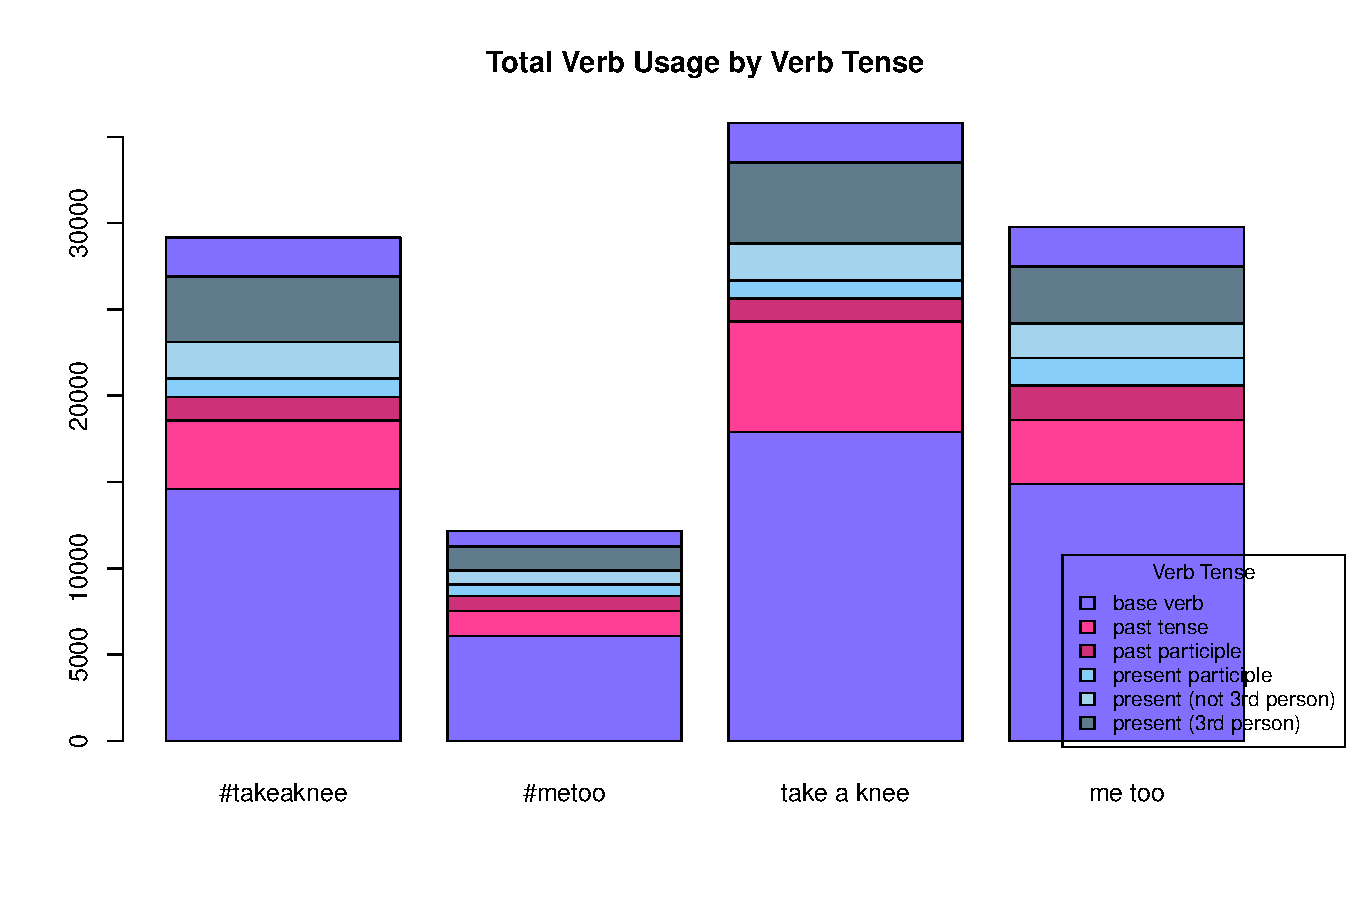
\includegraphics{figure/get_plot_verb_types_stacked-1.pdf}


\end{document}
